\chapter{Baze u bioinformatici} % Main chapter title

\label{Baze} % For referencing 


Automatizacija bioloških i hemijskih analiza početkom 21 veka omogućila je
ubrzanu i paralelnu analizu velikog broja uzoraka. Ove tehnologije žargonski su
poznate kao \keyword{tehnologije velike propusnosti} \en{high throughput
technology }. Primera radi tehnologije \keyword{sekvenciranja nove generacije}
\en{Next-Generation Sequencing} ili skraćeno \keyword{NGS} neprekidno napreduju
spuštajući cenu procedure i eksponencijalno povećavajući količinu dostupnih
sekvenci. Da bi se razumeo uticaj NGS tehnologije razmotrimo sledeći tok
događaja.  Od sveže sekvencionisanih nepoznatih genoma predviđaju se
potencijalni geni, od gena potencijalne proteinske sekvence.  Dobijene
proteinske sekvence mogu se dalje klasterovati u familije, automatski
anotirati, predviđati im se struktura, osobine itd.  Zatim moguće je vršiti
analize za generisanje novih bioloških znanja. Povezanost između funkcije i
neuređenosti proteina je jedan primer biološkog znanja. Dakle generisanje novih
informacija u jednoj oblasti (u ovom slučaju genomici) propagira se u druge
oblasti bioinformatike. Ovo je samo jedan primer ali ilustruje 2 bitne stvari.
\begin{enumerate}
  \item Informacije eksponencijalno rastu uvodeći čitavu oblast
    \keyword{omike}\footnote{termin objedinjuje gen\textbf{omiku}, proteomiku,
    transkriptomiku, glikomiku...} \en{omics}  u teritoriju \en{Big
  Data}\parencite{Chen2017}. (U našem radu pažljivo su odabrani podaci malog
  obima kako bi se izbegao ovaj scenario i sve analize su urađene na klasičnom
  kućnom računaru.)
  % \item U bioinformatici podaci su veoma povezani. 
  \item Biološki podaci su veoma povezani.
\end{enumerate}

Povezanost podataka preslikava se na baze. Većina baza je usko specijalizovana
za jedan tip informacije ili jedan organizam, ali zato sadrži reference ka
drugim (spoljnim) bazama, naučnim radovima ili  manje formalnim ali
informativnim resursima (veb strane, vikipedija, itd...). Specijalne baze kao
što je UniProtKB, pored primarnog sadržaja održavaju i veliki broj referenci
(dbxref) pokušavajući da međusobno povežu sve dostupne informacije. Konkrentno
UniprotKB (feb. 2018) održava reference ka čak 164 različite
baze\footnote{\url{www.uniprot.org/docs/dbxref}}.  Dakle bioinformatika kao
disciplina podrazumeva da će analize biti vršena kombinacijom informacija
nekoliko različitih baza.  Zbog raznovrsnosti i svrhe prikupljenih informacija
postoji veliki broj kategorija\footnote{Baze ne pripadaju ekskluzivno samo
jednoj kategoriji}(vrsta) baza.  Na adresi
\url{www.proteininformationresource.org/staff/chenc/MiMB/dbSummary2015.html}
kategorizovane su i prikazane kvalitenije proteinski orijentisane baza
(prikazana lista nipošto nije konačna)\parencite{Chen2017}. Za naše
istraživanje bile su potrebne naredne tri kategorije:

\begin{itemize}
  \item Baze sekvenci.\\ 
        Ove baze teoretski sadrže sve poznate sekvence i kontrolišu dodeljivanje 
        identifikacionog broja sekvence.
    \begin{itemize}
      \item Proteinske sekvence: UniProtKB
      \item DNK sekvence: (EMBL, GenBank, DDBJ)
    \end{itemize}
  \item Baze strukture: DisProt, D2P2, MobiDB, (PDB), ...
  \item Baze homologija: Gene Ontology, (Protein Ontology)
\end{itemize}


\section{UniProtKB/Svis-Prot}
\label{svis-prot}

\keyword{UniProt} skraćeno od \en{Universal Protein Resource} je konzorcijum
nastao 2002 god. izmedju tri organizacije: Evropski Bioinformatički
Institut (EBI), Švajcarski institut za Bioinformatiku (SIB) i Resurs
Proteinskih Informacija (PIR).  ''Misija UniProt-a je da naučnoj zajednici
obezbedi sveobuhvatan, visokokvalitetan i slobodno dostupan resurs proteinskih
sekvenci i funkcionalnih informacija.''\footnote{\url{www.uniprot.org}} 


Uniprot obuhvata nekoliko baza i podbaza sa striktno definisanim tokom
informacija \ref{fig:uniprot_overview}. Od prikazanih najbitnija je
\keyword{UniprotKB} \en{UniProt Knowledge Base} sačinjena od 2 podbaze.

\begin{figure}[h!]
  \centering
  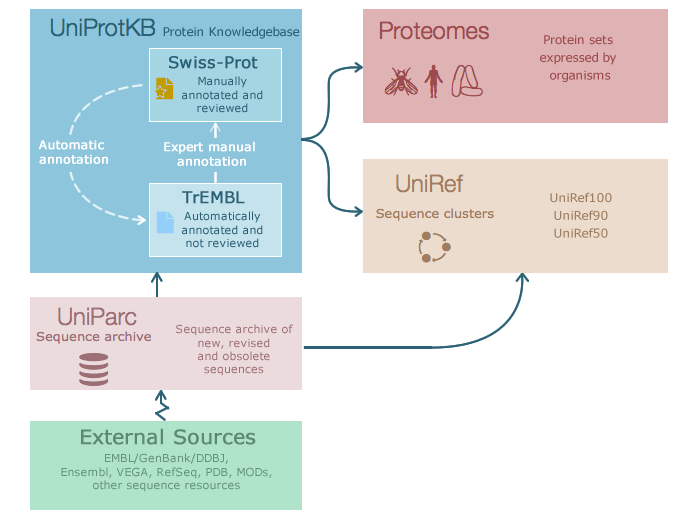
\includegraphics[width=0.8\linewidth]{uniprot_overview.png}
  \caption{Šematski prikaz povezanosti UniProt baza \ref{}}
  \label{fig:uniprot_overview}
\end{figure}

\begin{enumerate}
  \item \keyword{Svis-Prot} \en{Swiss-Prot} sadrži visoko kvalitetne anotacije
    \keyword{ne redundantnih}\ref{red} proteinskih sekvenci.
    Informacije o sekvenci su dobijene iz postojeće literature a kompjuterski
    predviđene anotacije su ručno proverene. Svis-Prot kao baza postoji preko
    30 godina.

  \item TrEMBL \en{Translated EMBL} je nadskup Svis-Prot sekvenci čije su
    sekvence dobijene prevođenjem EMBL nukleinskih sekvenci ali još nisu stigle
    da budu ručno  proverene. Ove sekvence su redundantne i njihova obimnost
    posledica je masovne primene NGS tehnologija. U februaru 2018. god TrEMBLE
    sadržao je 107,627,435 sekvenci što je oko 200 puta više u poređenju sa
    556,568 ručno proverenih Svis-Prot sekvenci. Sve nove sekvence prvo ulaze u
    sastav TrEMBL da bi ručnom proverom napredovale u Svis-Prot što je donekle
    prikazano grafikom \ref{fig:uniprot_overview}.
\end{enumerate}





Distribucije Svis-Prot baze dostupne su u nekoliko tekstualnih formata: ravna
datoteka \en{flat file}, XML, RDF/XML.  Ravni tekstualni format zbog
standardizacije prati format EMBL\parencite{embl} baze
\parencite{svisprot2003}.  Unos u bazu se zove \keyword{slog} \en{record} i
sadrži sve informacije vezane za jedan protein. Jedan slog ilustrovaćemo
uprošćenim primerom\ref{txt:slog} u formatu ravne datoteke na kome ilustrujemo
ključne osobine Svis-Prot baze:

\lstset{ 
  basicstyle=\footnotesize\ttfamily,        % the size of the fonts that are used for the code
  captionpos=b,                    % sets the caption-position to bottom
  commentstyle=\color{mygreen},    % comment style
  deletekeywords={...},            % if you want to delete keywords from the given language
  escapeinside={\%*}{*)},          % if you want to add LaTeX within your code
  extendedchars=true,              % does not work with UTF-8
  keywordstyle=\color{blue},       % keyword styli
  % language=Octave,                 % the language of the code
  morekeywords={ID, AC, PE, KW, GO, SQ}, % if you want to add more keywords to the set
  numbers=left,                    % where to put the line-numbers; 
  numbersep=5pt,                   % how far the line-numbers are from the code
  numberstyle=\color{mygray}, % the style that is used for the line-numbers
  % rulecolor=\color{black},         % if not set, the frame-color may be changed on line-breaks within not-black text (e.g. comments (green here))
  showstringspaces=false,          % underline spaces within strings only
}

\begin{figure}[h!]
  \label{txt:slog}
  \centering

\begin{lstlisting}
ID   ACSA_DROME              Reviewed;         670 AA.  | ime sloga, info
AC   Q9VP61; Q24226; Q8IH30; Q9VP60;                    | identifikacija
DT   19-SEP-2003, integrated into UniProtKB/Swiss-Prot. | ulazak u Svis-Prot
DT   01-MAY-2000, sequence version 1.                   | ulazak u TrEMBL
DT   25-OCT-2017, entry version 116.                    | poslednje 
                                                          osvezavanje sloga
\end{lstlisting}
\begin{lstlisting}[firstnumber=7,   basicstyle=\footnotesize\ttfamily\color{gray}]
DE   RecName: Full=Acetyl-coenzyme A synthetase;        |
DE            EC=6.2.1.1;                               |
DE   AltName: Full=Acetyl-CoA synthetase;               |
DE            Short=ACS;                                |
GN   Name=AcCoAS; ORFNames=CG9390;                      |
OS   Drosophila melanogaster (Fruit fly).               | Taksonomija
OC   Eukaryota; Metazoa; Ecdysozoa; Arthropoda; Hexap...|
OC   Pterygota; Neoptera; Holometabola; Diptera; Brac...|
OC   Ephydroidea; Drosophilidae; Drosophila; Sophopho...|
OX   NCBI_TaxID=7227 {ECO:0000312|EMBL:AAL90278.1};     |
                                                        
RN   [1] {ECO:0000305}                                  | Prva referenca
RP   NUCLEOTIDE SEQUENCE (ISOFORM B).                   | 
RA   Russell S.R., Heimbeck G.M., Carpenter A.T., Ash...| Autori
RT   "A Drosophila melanogaster acetyl-CoA-synthetase...| Naslov
RL   Submitted (NOV-1994) to the EMBL/GenBank/DDBJ da...|
RN   [2]                                                | Druga referenca              
...                                                     
CC   -!- FUNCTION: Activates acetate so that it can b...| Komentari
CC       synthesis or for energy generation.            |
CC       {ECO:0000250|UniProtKB:Q9NR19}.                |
CC   -!- CATALYTIC ACTIVITY: ATP + acetate + CoA = AM...|
...                                                     
\end{lstlisting}
\begin{lstlisting}[firstnumber=30]
DR   EMBL; Z46786; CAA86738.1; ALT_SEQ; mRNA.           | reference ka
DR   EMBL; AE014296; AAF51695.2; -; Genomic_DNA.        | drugim bazama 
...                                                     | (dbxref)
DR   ExpressionAtlas; Q9VP61; differential.             |
DR   Genevisible; Q9VP61; DM.                           |
DR   GO; GO:0005737; C:cytoplasm; IEA:UniProtKB-SubCell.| GO termin <----
DR   GO; GO:0003987; F:acetate-CoA ligase activity; I...| GO termin <----
...                                                     |
\end{lstlisting}
\begin{lstlisting}[firstnumber=38]
PE   2: Evidence at transcript level;
KW   Alternative splicing; ATP-binding; Complete proteome; Cytoplasm; 
KW   Ligase; Nucleotide-binding; Reference proteome.                  
FT   CHAIN         1    670       Acetyl-coenzyme A synthetase.
FT                                /FTId=PRO_0000208425.
FT   VAR_SEQ       1    146       Missing (in isoform B).
FT                                {ECO:0000303|PubMed:12537569}.
FT                                /FTId=VSP_008310.
FT   CONFLICT    227    227       C -> S (in Ref. 1; CAA86738).
FT                                {ECO:0000305}.
SQ   SEQUENCE   670 AA;  75960 MW;  CE24364755CDBFFC CRC64;
     MPAEKSIYDP NPAISQNAYI SSFEEYQKFY QESLDNPAEF WSRVAKQFHW ETPADQDKFL
...
     KKMVRERIGP FAMPDVIQNA PGLPKTRSGK IMRRVLRKIA VNDRNVGDTS TLADEQIVEQ
     LFANRPVEAK
//  <--- oznacava kraj sloga
\end{lstlisting}
\caption{Uprošćen primer sloga (unosa) u Svis-Prot}
\end{figure}



\begin{enumerate}
  \item Ime sloga \keyword{ID} \en{entery name} je mnemonički zapis koji kodira
    taksonomske informacije o genu i proteinu. ID je podložan promenama tokom vremena
    i ne može se koristiti kao identifikator \parencite{www_svisprot}.
  \item Identifikacioni broj predstavlja \keyword{AC} \en{accession number}.
    Prvi u listi identifikatora naziva se \keyword{primarni} i služi da
    jednoznačno odredi slog. Ostatak identifikatora su tzv. \keyword{sekundarani AC} i
    nastaju iz dva moguća razloga: \parencite{svisprot2003, www_svisprot}
    \begin{itemize}
      \item Unifikacija postojećih proteina u jedan novi slog. 
      \item Specijalizacija jednog proteina u više različitih.
    \end{itemize}
    U oba slučaja stari (primarni) AC se zadržava kao sekundarni AC u novom slogu.

  \item Za razliku od TrEML, GO mapiranje za Svis-Prot sekvence određuju se ručno\parencite{www_svisprot}.

  \item \keyword{Ključne reči} \en{keywords} označene \keyword{KW} opisuju
    hijearhisku strukturu kontrolisanog vokabulara namenjenog opisivanju
    funkcije proteina. Postoji 10 kategorija ključnih reči od kojih je za naše
    istraživanje bitna "Molekulska funkcija"\parencite{svisprot2003}.  Za razliku od GO termina ključne
    reči prligaođene su opisivanju sadržaja isključivo Svis-Prot proteina\parencite{www_svisprot}.

  \item Sekvenca \keyword{SQ} u slogu poznata je kao \keyword{kanonska}
    \en{canonical} sekvenca. Kanonska sekvenca predstavlja konsenzus sekvencu
    produkta (protein) gena jedne vrste organizma.  \keyword{FT}
    linije čuvaju različite osobine kanonske sekvence uključujući i razlike u
    odnosu na izoforme\footnote{Izoformi su alternativni oblici sekvence
      nastali usled: \en{ alterntive promoter usage, alternative splicing,
    alternative initiation and ribosomal frameshifiting} } sekvence.  U našoj
    analizi korišćena je isključivo kanonska sekvenca. Detaljan opis pravila za
    biranje kanonske sekvence može se naći na \parencite{www_svisprot}.

  \item
    \label{red}
    Svis-Prot je \keyword{minimalno redundantna} u smislu da svi proteini
    kodirani jednim genom, jedne vrste su predstavljeni jednim slogom. Svi
    izoformi su grupisani pod jedan slog i jednu kanonsku sekvencu\parencite{nonRedundant}.

  \item Postojnost proteina \keyword{PE} \en{Protein existance} opisuje stepen
    sigurnosti da protein postoji. \ref{fig:PE}

  \clearpage


  \item
    Swis-Prot takđe vrši predikcije neuređenih regiona:  koristeći DISOPRED2
    and CLADIST prediktor \parencite{meng_c2017}\\ Međutim ove informacije
    postale su irelevantne pojavom baza MobiDB i D2P2 koje razmatramo u
    sekcijama ispod.

  \item Zanimljiva zapažanja globalne statistike:
    \begin{itemize}
      \item Najzastupljenije sekvence su kraće od 500 aminokiselina.
      \item Postojnost oko 70\% proteina potvrđeno je homologijom.
      \item Zastupljeno je preko 1000 različitih organizama međutim
        većina Svis-Prot sekvenci pripada malom broju model organizama.
    \end{itemize}
      


\end{enumerate}

\begin{figure}[h!]
  \centering
  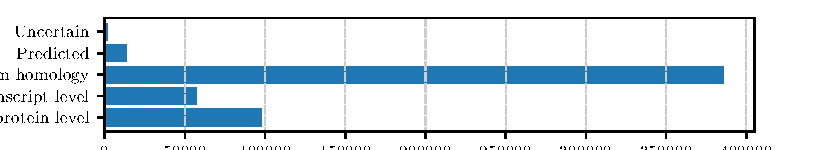
\includegraphics[]{plots/PE.pdf}
  \label{fig:PE}
  \caption{Histogram nivoa pouzdanosti Svis-Prot proteina}
\end{figure}

\section{Disprot}

Baza proteinskog neuređenja \en{Database of protein Disorder (DisProt)}

\section{D2P2 i MobiDB}

Baze prdviđenog neuređenja proteinskih sekvenci


\section{Ontologije Gena}


\keyword{Ontologija Gena} \en{Gene Ontology} ili skraćeno \keyword{GO}, 
predstavlja izračunato znanje o funkciji gena odnosno genskog
produkta (protein, nekodirajuća RNK ili makromolekulski kompleks)
\parencite{GO2016}.
GO baza sačinjena je iz dve komponente:
\begin{enumerate}
  \item \keyword{Ontologije gena}.
  \item \keyword{GO anotacije} tj. antoacije genskog produkta \keyword{GO terminom}. U našoj
    analizi anotacije su preuzete iz Svis-Prot baze\footnote{Ali Svis-Prot koristi anotacije iz ontologije gena}.
\end{enumerate}

Ontologija gena definiše univerzum termina, takozvanih \keyword{GO termina}
\en{GO terms} i njihove međusobne relacije. GO termini predstavljaju biološke
termine (koncepte) koji opisuju funkciju. Ontologija gena sagledava funkciju
genskog produkta iz tri aspekta koji se u terminologiji ontologija nazivaju
imenski prostori \en{namespace}:
\begin{itemize}
  \item \keyword{Molekulska funkcija (MF)} je biohemijska aktivnost (uključujući
    specifično vezivanje za ligande ili strukture) genskog produkta.
  \item \keyword{Ćelijske komponente  (CC)} se odnosi na mesto u ćeliji gde je
    genski produkt aktivan.
  \item \keyword{Biološki procesi (BP)} se odnosi na proces kome genski produkt
    doprinosi.
\end{itemize}

Inspirisani sličnošću prva tri sekvencisana eukariotska organizma, GO projekat
nastao je sa ciljem da  unifikuje biologiju pod jedan univerzum termina za opis
genskih proizvoda svih vrsta organizama\parencite{GO2000}. Ovaj ideal je najveća
razlika u odnosu na kontrolisani vokabular Svis-Prot ključnih reči koji je
prilagođen za opis samo proteina sadržanih u Svis-Prot bazi.

Suštinu ontologije čine relacije između termina i pravila dedukcije koja se nad
njima mogu primenjivati. Osnovnu strukturu ontologije čini direktni aciklički
graf \en{DAG} obrazovan roditeljskom vezom (relacijom) \keyword{is\_a}. Prateći
ovu relaciju termini jednog imenskog prostora recimo MF neće nikad preći u
druga dva CC i BP.  Ontologija stoga ima tri korena čvora MF, CC i BP
\parencite{go_struktura}. Primer strukture prikazan je na
slici \ref{fig:kinase}.  Pored \keyword{is\_a} postoje dodatne relacije od kojih
su najčešće \footnote{Vremenom se ontologija proširuje novim tipovima relacije
koje su van okvira ovog rada.}:

\begin{itemize}
  \item \keyword{part\_of}  - je deo  (ne znači da je uvek deo vezanog termina)
  \item \keyword{has\_part} - ima deo (deo uvek postoji)
  \item \keyword{regulates} - pozitivna ili negativna regulacija
  \item \keyword{positvely\_regulates} - pozitivna regulacija  
    (\keyword{is\_a} termin koji reguliše)
  \item \keyword{negatively\_regulates} - negativna regulacija 
    (\keyword{is\_a} termin koji reguliše)
\end{itemize}

\begin{figure}[h!]
  \centering
  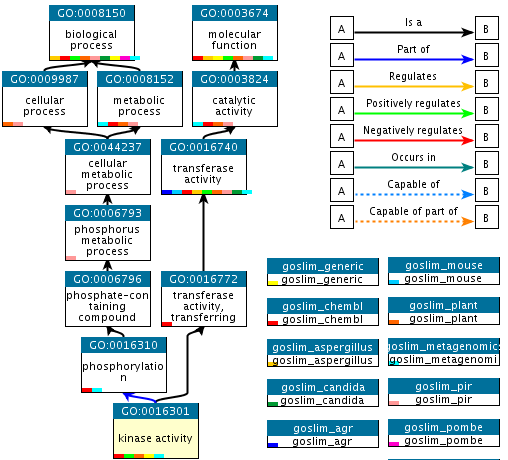
\includegraphics[width=0.8\linewidth]{img/kinase.png}
  \caption{Struktura ontologije}
  \label{fig:kinase}
\end{figure}

Svaka veza (relacija) ima strogo definisana pravila kompozicije koja omogućavaju
automatsko rezonovanje. Recimo relacija \keyword{is\_a} ima svojstvo
tranzitivnosti\parencite{is_a}:
\begin{verbatim}
  A is_a    B  /\  B is_A C   =>    A is_a    C           
  A part_of B  /\  B is_A C   =>    A part_of C
\end{verbatim}

Siže pravila rezonovanja prikazano je na slici \ref{fig:relations}.

Ontologije su dostupne u nekoliko formata. U našem radu korišćen je ravni
\file{.obo} format.  Pored njega treba naglasiti postojanje \file{RDF/XML} i
\file{OWL} verzija.  Ove verzije namenjene su automatskom rezonovanju unutar
specijalizovanih softvere i upitnih jezika \footnote{U našem radu korišćena je
Neo4j grafovska bazu što naš postupak rezonovanja čini eksplicitnim} (protégé,
SPARQL, ...).

\begin{figure}[h!]
  \centering
  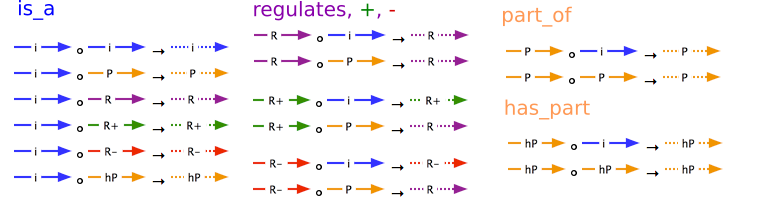
\includegraphics[width=1.0\linewidth]{relations.png}
  \caption{Pravila rezonovanja (isprekidane relacije su rezultat)}
  \label{fig:relations}
\end{figure}

GO termin može biti zastareo u kom slučaju se relacijom \keyword{replaced\_by}
pokazuje na noviji termin. Relacija \keyword{consider} ukazuju na
postojanje mogućih ekvivalentnih termina. Pored glavnog univerzuma postoje i
podskupovi \footnote{Uglavnom ovi podskupovi predstavljaju model organizme}
termina (GO slim) prikazani u donjem desnom delu slike \ref{fig:kinase}.


\subsection{molekulska funkcija}
TODO, treba proučiti \parencite{go_mf} možda nešto saznam o kvalitetu anotacija
u Svis-Prot bazi.










